\documentclass[a4paper,11pt]{article}
\usepackage[mag=1000]{newlistok}
\usepackage{tikz}
\usetikzlibrary{calc}

\УвеличитьШирину{1.4truecm}
\УвеличитьВысоту{2.5truecm}

\Заголовок{Предел последовательности}
\НомерЛистка{32}
\ДатаЛистка{27.02 -- 13.03.2019}
\Оценки{43/36/19}
\renewcommand{\spacer}{\vspace{1.3pt}}

\begin{document}

%\scalebox{.89}{\vbox{%
%\ncopy{1}{

\СоздатьЗаголовок

\опр %Пусть $\varepsilon>0$. % --- произвольное положительное число.
\выд{Окрестность} точки $a$ %(где $\varepsilon>0$)
--- это %называют
любой интервал, содержащий точку $a$.
%$(a-\varepsilon, a+\varepsilon)$. % = \{ x: |x-a| < \varepsilon \}$.
Обозначение: ${\cal U(\it a)}$. % _\varepsilon(a)$.
\копр

\задача
Докажите, что любые две различные точки на прямой имеют непересекающиеся
окрестности.
\кзадача

\опр \label{limit3} Число $a$ называют \выд{пределом последовательности}
$(x_n)$ и пишут $\lim\limits_{n \to \infty} x_n = a$, если %последовательность $(x_n-a)$ является бесконечно малой.
%\задача
%Докажите, что последовательность $(x_n)$ сходится к числу $a$
%тогда и только тогда, когда
выполнено любое из следующих трёх эквивалентных определений:\\
$\bullet$ $(x_n)$ можно представить в виде
$x_n=a+\alpha_n$, где $(\alpha_n)$ --- бесконечно малая
последовательность;\\
$\bullet$ любая окрестность точки $a$ является ловушкой для $(x_n)$;\\
$\bullet$ для каждого числа $\varepsilon>0$ найд\"ется такое число $N$,
что при любом натуральном $n\geq N$ выполнено $|x_n-a|<\varepsilon$.\\
%\кзадача
%Обозначение: $\lim\limits_{n \to \infty} x_n = a$.
Говорят также, что \выд{$(x_n)$ стремится к $a$ при $n$,
стремящемся к бесконечности}
(и пишут $x_n \to a$ при~\hbox{$n \to \infty$)}.
%или говорят, что \выд{$(x_n)$ сходится к $a$}.
\копр

\задача %Докажите, что
Может ли последовательность
%не может
иметь более одного предела?
\кзадача


\пзадача
Запишите % утверждения,
без отрицания:
\вСтрочку
\пункт
%Напишите, что значит, что
\лк число
$a$ не предел %последовательности
$(x_n)$\пк;
\пункт
%Напишите, что значит, что
\лк %последовательность
$(x_n)$ не имеет~предела\пк.
\кзадача

%\задача
%Последовательность имеет предел. Обязательно ли она ограничена?
%\кзадача

\задача
%Последовательность имеет ненулевой предел.
Пусть $\lim\limits_{n \to \infty}x_n>0$. %положителен.
Верно ли, что
\пункт $\!\!x_n>0$ при $n\gg0$;
%все члены $(x_n)$, начиная с некоторого, положительны;\\
\пункт $\!\!(1/x_n)$ ограничена (если определена)?
%отличны от нуля и имеют один и тот же знак?
\кзадача

%\задача Последовательность $(x_n)$ имеет предел $a$.
%\вСтрочку
%\пункт Обязательно ли $(x_n)$ ограничена?\\
%\пункт Пусть $a>0$ и все члены $(x_n)$ положительны.
%Докажите, что последовательность $(1/x_n)$ ограничена.
%\кзадача

%\задача Предел $(x_n)$ равен $a$.
%Обязательно ли ограничена
%\вСтрочку
%\пункт $\!\!(x_n)$;
%\пункт $\!\!(1/x_n)$, если $a>0$ и члены $(x_n)$~\hbox{положительны?}
%Докажите, что последовательность ограничена.
%\кзадача

\ввпзадача
Пусть
$\lim\limits_{n \to \infty} x_n = a$,
$\lim\limits_{n \to \infty} y_n = b$.
%Докажите:
Найти
\вСтрочку
%\пункт $\lim\limits_{n \to \infty} (x_n \pm y_n)= a\pm b$;
%\пункт $\lim\limits_{n \to \infty} (x_n\cdot y_n) = ab$;\\
%\пункт если $b\ne0$ и все элементы
%последовательности $(y_n)$ отличны от нуля, то
%$\lim\limits_{n \to \infty} (x_n/y_n) = a/b$.
\пункт $\lim\limits_{n \to \infty} x_n \pm y_n$;
\пункт $\lim\limits_{n \to \infty} x_n\cdot y_n$;
\спункт
$\lim\limits_{n \to \infty}\dfrac{x_n}{y_n}$, если $b\ne0$.
%если $b\ne0$ и все элементы
%последовательности $(y_n)$ отличны от нуля, то
\кзадача

\задача
\вСтрочку
\пункт Пусть
$(x_n)$ %известно, что она
имеет предел.
Докажите, что %последовательность
$(x_{n+1}-x_n)$ бесконечно малая.
\пункт Верно ли обратное?
\кзадача

\пзадача Найдите предел, если он есть:
\вСтрочку
%\пункт $x_n=1+(-1)^n$;
\пункт \hbox{$1+(-0,1)^n$;}
\пункт $\dfrac{n}{n+1}$;
%\пункт $x_n=n/(n+1)$;
\пункт $(-1)^n$;
%\пункт $x_n=\dfrac{2^n-1}{2^n+1}$;
\пункт $\dfrac{2^n-1}{2^n+1}$;
\пункт $\sqrt{n+1}-\sqrt{n}$;\\
\пункт $\sqrt{n^2+n}-n$;
\пункт $1+q+\ldots+q^{n}$, где $|q|<1$;
\пункт $\dfrac{1+3+\ldots+3^n}{5^{n}}$;
%\пункт $\!\!\dfrac{n^2-n+1}{n^2}$;
%\пункт $x_n=\sqrt{n^2+n}-\sqrt{n}$;
\пункт $\sqrt[n]{2}$;
\пункт $\sqrt[n]{2^n+3^n}$;
\пункт $\dfrac{n^{50}}{2^n}$;
\пункт $\root n \of n$.
\кзадача


\задача
Может ли последовательность без наименьшего и
наибольшего членов иметь предел?
\кзадача

%\задача Пусть $A(x)=a_k x^k+\ldots+a_1x+a_0$ и
%$B(x)=b_m x^m+\ldots+b_1x+b_0$ --- многочлены степеней $k$ и $m$
%соответственно. Найдите пределы:
%\вСтрочку
%\пункт $\lim\limits_{n \to \infty}A(n)/n^k$;
%\пункт $\lim\limits_{n \to \infty}A(n)/B(n)$.
%\кзадача


\пзадача Найдите: % пределы: % последовательностей:
\вСтрочку
\пункт $\displaystyle{\lim\limits_{n \to \infty}\frac{n^2+n+1}{4n^2}}$
\пункт $\displaystyle{\lim\limits_{n \to \infty}\frac{n^2+2n-2}{n^3+n}}$;
\пункт $\displaystyle{\lim\limits_{n \to \infty}\frac{n^9-n^4+1}{2n^9+7n-5}}$;
\пункт $\displaystyle{\lim\limits_{n \to \infty}\frac{C^{50}_n}{n^{50}}}$.
\кзадача

\vspace*{1mm}

%\задача Про последовательность $(x_n)$ известно, что она
%имеет предел и содержит бесконечно много положительных
%и бесконечно много отрицательных членов.
%Докажите, что %эта последовательность
%$(x_n)$ бесконечно малая.
%\кзадача


\задача
Пусть $\lim\limits_{n \to \infty} x_n =a$, $\lim\limits_{n \to
\infty} y_n = b$ и $x_n>y_n$ при $n\in\N$.
Верно ли, что
\вСтрочку
\пункт $a>b$;
\пункт $a\geq b$?
\кзадача


\пзадача
Обобщите теорему о двух милиционерах из листка 31
на последовательности, имеющие предел.
\кзадача

%\задача[\лк Теорема о двух милиционерах\пк]
%Пусть $\lim\limits_{n \to \infty} x_n =\lim\limits_{n \to
%\infty} y_n = а$, и последовательность $(z_n)$ такова,
%что $x_n\leq z_n\leq y_n$ при любом номере $n$.  Докажите,
%что $\lim\limits_{n \to \infty} z_n = a$.
%\кзадача

%\задача Известно, что $\lim\limits_{n \to \infty} x_n = 1$.
%Найдите предел последовательности $(y_n)$, если\\
%\вСтрочку
%\пункт $y_n=(2x_n-1)/(x_n+1)$;
%\пункт $y_n=(x_n^2+x_n-2)/(x_n-1)$;
%\пункт $y_n=\sqrt{x_n}$;
%\спункт $y_n=(x_1+\ldots+x_n)/n$.
%\кзадача

%\vspace*{-2.1truemm}

\задача Пусть $\lim\limits_{n \to \infty}\! x_n = 1$.
Найти
\вСтрочку
\пункт  $\displaystyle{\lim\limits_{n \to \infty}\!\frac{x_n^2}{7}}$;
\пункт  $\displaystyle{\lim\limits_{n \to \infty}\!\frac{x_n^2+x_n-2}{x_n-1}}$;
\пункт  $\lim\limits_{n \to \infty}\!\sqrt{x_n}$;
\спункт $\displaystyle{\lim\limits_{n \to \infty}\!\frac{x_1+\ldots+x_n}n}$.
\кзадача

%\задача Для вычисления квадратного корня из положительного
%числа $a$ можно пользоваться следующим методом
%последовательных приближений. Возьмите любое положительное число
%$x_0$ и постройте последовательность по такому закону:
%$x_{n+1}=0,5\cdot(x_n+a/x_n).$
%\сНовойСтроки
%\вСтрочку
%\пункт
%Докажите, что $\lim\limits_{n\to\infty}x_n=\sqrt a$.\\
%\спункт Сколько понадобится последовательных приближений,
%чтобы найти $\sqrt{10}$ с точностью до $0,0001$,
%если в качестве первого приближения взять $x_0=3$?
%\кзадача


%\задача Про последовательность $(x_n)$ известно, что она
%имеет ненулевой предел и состоит из ненулевых членов.
%Докажите, что последовательность $(1/x_n)$ ограничена.
%\кзадача

%\задача Является ли бесконечно малой последовательность $(x_n)$, где
%%$x_n=\dfrac{n^{100}}{7^n}$?
%$x_n=n^{100}/7^n$?
%\кзадача


\УстановитьГраницы{0cm}{3.2cm}
\пзадача
\righttikz{0mm}{0mm}{%
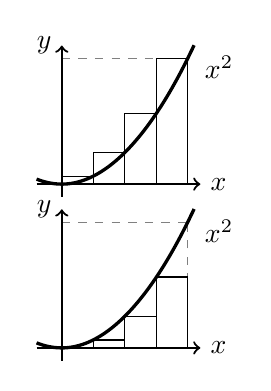
\begin{tikzpicture}[scale=1.6]
\begin{scope}
  \draw[style=help lines, dashed] (0,0) grid (1,1);
  \draw[->, thick] (-0.2,0) -- (1.1,0) node[right] {$x$};
  \draw[->, thick] (0,-0.1) -- (0,1.1) node[left] {$y$};
  \draw[very thick] (-.2,.04) parabola bend (0,0) (1.05,1.1025) node[below right] {$x^2$};
  \draw (0,0) rectangle (0.25, 0.0625);
  \draw (0.25,0) rectangle (0.5, 0.25);
  \draw (0.5,0) rectangle (0.75, 0.5625);
  \draw (0.75,0) rectangle (1.0, 1);
\end{scope}
\begin{scope}[yshift=-1.3cm]
  \draw[style=help lines, dashed] (0,0) grid (1,1);
  \draw[->, thick] (-0.2,0) -- (1.1,0) node[right] {$x$};
  \draw[->, thick] (0,-0.1) -- (0,1.1) node[left] {$y$};
  \draw[very thick] (-.2,.04) parabola bend (0,0) (1.05,1.1025) node[below right] {$x^2$};
  \draw (0.25,0) rectangle (0.5, 0.0625);
  \draw (0.5,0) rectangle (0.75, 0.25);
  \draw (0.75,0) rectangle (1, 0.5625);
\end{scope}
\end{tikzpicture}
}
\пункт
Дана фигура, ограниченная графиком
функции $y=x^2$, осью $Ox$ и прямой $x=1$. Разобь\"ем
отрезок $[0,1]$ на $n$ равных частей и построим на каждой
части прямоугольник так, чтобы его правая верхняя вершина
лежала на графике (см.~рис. справа).
Сумму
площадей прямоугольников обозначим $S_n$.
%Найдите $\lim\limits_{n \to\infty}(S_n)$.\\
Найдите предел $(S_n)$ при $n \to \infty$.\\
\пункт Построим прямоугольники так, чтобы
их левые верхние вершины лежали на графике. % (см.~рис.).
%Соответствующую
Сумму их площадей~обозначим $s_n$. Докажите,
что %последовательность
$(s_n)$ стре\-мит\-ся к тому же числу,
что и $(S_n)$ (это \выд{площадь}
нашей фигуры).
%\спункт Найдите площадь фигуры, ограниченной графиком
%функции $y=x^k$, осью $Ox$ и прямой $x=1$ ($k$ ---
%фиксированное натуральное число).
\спункт Решите ту же задачу для функции $y=x^k$, где~\hbox{$k\in\N$.}
\ВосстановитьГраницы
\кзадача




%\задача Найдите предел последовательности $(a_n)$, где
%%$\displaystyle{a_n=\frac12+\frac2{2^2}+\frac3{2^3}+\ldots+\frac{n}{2^n}}$.
%$a_n=1/2+2/2^2+3/2^3+\ldots+n/2^n$.
%\кзадача

%\задача
%Пусть $x_n=a_1/1+a_2/2+\dots+a_n/n$, где $a_n=1$, если
%в десятичной записи числа $n$ нет цифры 9, и $a_n=0$
%иначе. Имеет ли эта последовательность предел?
%\кзадача


%\сзадача
%Из клетчатой плоскости вырезали клетки, обе координаты которых
%делятся на 10. Можно ли оставшуюся часть плоскости разрезать
%на доминошки (каждая состоит из двух соседних клеток)?
%\кзадача


% Посл и пределы


%}}}


% \раздел{***}
%
% \vspace*{-2mm}

\задача
При каких натуральных $k$ выполнено равенство
$
\displaystyle{
\lim\limits_{n\rightarrow\infty}\frac{n^k-(n-1)^k}{n^{2018}}=2019?}
$
\кзадача



\задача Последовательность $(x_n)$ построена так: первый член выбирается произвольно, а каждый следующий находится по формуле $x_{n+1}=ax_n+1$. При каких $a$ последовательность $(x_n)$ всегда будет иметь предел?
\кзадача

\пзадача
Пусть $x_n>0$ при $n\in\N$ и $\displaystyle{\lim\limits_{n \to \infty}\frac{x_{n+1}}{x_{n}}}=q$, где $q<1$.
% Последовательность $(x_n)$ положительна, а последовательность $(x_{n+1}/x_n)$ имеет пределом
% некоторое число, меньшее 1.
Докажите, что %последовательность
$(x_n)$ бесконечно малая.
\кзадача


\сзадача
Дано $m$ последовательностей, сумма которых
стремится к $m\alpha$, и сумма квадратов которых
стремится к $m\alpha^2$. Докажите, что каждая из этих
последовательность стремится к $\alpha$.
\кзадача







%\задача
%Первые два члена последовательности равны $0$ и $1$,
%а каждый следующий есть среднее арифметическое двух предыдущих.
%Найдите предел этой последовательности.
%\кзадача



\задача %С незапамятных врем\"ен
Издавна жители островов Чунга и Чанга раз в год
меняются~драгоцен\-ностями. Одновременно~жители Чунги привозят
половину своих драгоценностей на Чангу, а жители
Чанги %~одновре\-мен\-но привозят
треть своих драгоценностей на
Чунгу.
%Так продолжается .
Какая часть драгоценностей находится~на~каж\-дом острове?
(Общий набор драгоценностей постоянен.) %за это время %на островах не менялся.)
\кзадача

%\задача
%Последовательность $(a_n)$ состоит из
%ненулевых членов и имеет предел 0. Известно, что
%последовательность $(\frac{a_{n+1}}{a_n})$ имеет предел
%$\alpha$. Найдите все возможные значения $\alpha$.
%\кзадача


%\сзадача Петя вышел из дому и пош\"ел в школу.
%На полпути к школе он решил, что лучше пойти в кино, и
%свернул к кинотеатру. Пройдя половину пути, он
%захотел покататься на коньках и свернул к катку.
%Пройдя половину пути до катка, он подумал, что нужно
%вс\"е-таки учиться, и повернул к школе. Но на полпути
%к школе снова свернул к кинотеатру, и т.~д. Куда
%прид\"ет Петя, если будет так идти?
%\кзадача

\задача \пункт Петя шёл из дома в школу.
На полпути он решил, что болен, и
пошёл обратно. На полпути к дому ему стало лучше,
и он повернул в школу. На полпути к школе он решил, что
всё-же болен, и повернул домой. Но на полпути
к дому снова повернул к школе, и т.~д. Куда
придёт Петя?
\спункт В другой раз Петя на полпути к школе свернул к катку,
на полпути к катку свернул к дому, и т.д. Куда теперь придёт Петя?
% \пункт Петя шел из дома в школу.
% На полпути он решил, что лучше пойти в кино, и
% свернул к кинотеатру. На полпути к кинотеатру
% он повернул к катку.
% На полпути к катку он подумал, что надо же
% учиться, и повернул к школе. Но на полпути
% к ней снова свернул к кинотеатру, и т.~д.
%Куда прид\"ет Петя, если будет так идти?
\кзадача




%\задача Найдите предел последовательности $(a_n)$, где
%%$\displaystyle{a_n=\frac12+\frac2{2^2}+\frac3{2^3}+\ldots+\frac{n}{2^n}}$.
%$a_n=1/2+2/2^2+3/2^3+\ldots+n/2^n$.
%\кзадача

%\задача
%Пусть $x_n=a_1/1+a_2/2+\dots+a_n/n$, где $a_n=1$, если
%в десятичной записи числа $n$ нет цифры 9, и $a_n=0$
%иначе. Имеет ли эта последовательность предел?
%\кзадача

\задача
%Задача Кириллова о манной каше.
По кругу сидят $n$ ребят, у каждого по тарелке каши.
Каждую минуту одновременно %происходит перераспре
%Ежеминутно
каждый из ребят берет себе
по половине каши своих соседей. Сначала в тарелках было
$1, 2, \dots, n$ поварешек каши.
%Верно ли, что спустя достаточно большое время
%каши в тарелках будет примерно поровну? Решите задачу, если
Сколько каши будет в тарелках спустя достаточно долгое время, если
%\вСтрочку
\пункт $n=3$;
\пункт $n=4$;
\спункт $n\in\N$?\\
% \сспункт А если ребята сидят в вершинах графа
% и ежеминутно каждый делит свою кашу поровну между соседями?
\кзадача



\ЛичныйКондуит{0mm}{6mm}
% \GenXMLW

%\СделатьКондуит{4.1mm}{7.5mm}

\end{document}


\задача Для вычисления квадратного корня из положительного
числа $a$ можно пользоваться следующим методом
последовательных приближений. Возьмите любое положительное число
$x_0$ и постройте последовательность по такому закону:
$x_{n+1}=0,5\cdot(x_n+a/x_n).$\\
%\сНовойСтроки
%\вСтрочку
\пункт
Докажите, что $\lim\limits_{n\to\infty}x_n=\sqrt a$.\\
\спункт Сколько понадобится последовательных приближений,
чтобы найти $\sqrt{10}$ с точностью до $0,0001$,
если в качестве первого приближения взять $x_0=3$?
\кзадача


----------


\задача[\лк Теорема о двух милиционерах\пк]
Пусть $\lim\limits_{n \to \infty} x_n =\lim\limits_{n \to
\infty} y_n = а$, и последовательность $(z_n)$ такова,
что $x_n\leq z_n\leq y_n$ при любом номере $n$.  Докажите,
что $\lim\limits_{n \to \infty} z_n = a$.
\кзадача



\задача Пусть $A(x)=a_k x^k+\ldots+a_1x+a_0$ и
$B(x)=b_m x^m+\ldots+b_1x+b_0$ --- многочлены степеней $k$ и $m$
соответственно. Найдите:
\вСтрочку
\пункт $\lim\limits_{n \to \infty}A(n)/n^k$;
\пункт $\lim\limits_{n \to \infty}A(n)/B(n)$;
\пункт $\lim\limits_{n \to \infty}(S_k(n)/n^k-n/(k+1))$.
\кзадача

\сзадача Найдите %предел последовательности $(a_n)$, если\\
\вСтрочку
\пункт
$\displaystyle{
\lim\limits_{n\to\infty}
\left(\frac{1^k+2^k+\ldots+n^k}{n^k}-\frac{n}{k+1}\right)}$,
где $k\in\N$;
\пункт
$\displaystyle{\lim\limits_{n\to\infty}\frac{1^1+2^2+\ldots+n^n}{n^n}}$.
\кзадача

%\сзадача
%Дано $n$ последовательностей, сумма которых
%стремится к $n\alpha$, и сумма квадратов которых
%стремится к $n\alpha^2$. Докажите, что каждая из этих
%\кзадача

%\сзадача [Критерий Коши]
%Докажите, что последовательность $(x_n)$ сходится тогда и
%только тогда, когда выполнено условие
%$\quad\forall \varepsilon>0 \quad \exists k\in\N\quad \forall m,n\ge k
%\quad |x_m-x_n|<\varepsilon$.
%\кзадача



\ЛичныйКондуит{0mm}{56mm}

\end{document}

\задача Найдите ошибку в рассуждении:
%Рассмотрим последовательность
\лк Пусть $x_n=(n-1)/n$. Тогда
%С одной стороны,
$\lim\limits_{n \to \infty} x_n =
\lim\limits_{n \to \infty}(1-1/n)=1$.\break
С другой стороны,
$\lim\limits_{n \to \infty} x_n =
\lim\limits_{n \to \infty}(1/n)\cdot\lim\limits_{n \to \infty}(n-1)
= 0\cdot\lim\limits_{n \to \infty} (n-1)= 0$.
Отсюда $0=1$.\пк
\кзадача

